\documentclass[11pt]{article}

\usepackage{../handout}
\usepackage{amsmath}
\usepackage{graphicx}

% Side margins:
% Actual margin is 1 in + this number
\oddsidemargin -0.25in
\evensidemargin -0.25in

% Text width:
\textwidth 6.9in

% Top margin:
% Actual margin is 1.5 in + this number
\topmargin -.3in

% Text height:
\textheight 8.7in


\begin{document}
\handout{13}{6}{Solutions to Written Assignment 4}

\begin{enumerate}

\item
\label{cond}
Suppose that we want to add the following conditional expression to
Cool.
\vspace{-0.5\baselineskip}
\begin{verbatim}
cond <p1> => <e1>; <p2> => <e2>; ... ; <pn> => <en>; dnoc
\end{verbatim}

\vspace{-0.5\baselineskip}
There must be at least one predicate and expression pair (that is,
$n \geq 1$).  The evaluation of a \texttt{cond} expression begins with
the evaluation of the predicate \texttt{<p1>}, which must have static
type \texttt{Bool}.  If \texttt{<p1>} evaluates to \texttt{true}, then
\texttt{<e1>} is evaluated, and the evaluation of the \texttt{cond}
expression is complete.  If \texttt{<p1>} evaluates to \texttt{false},
then \texttt{<p2>} is evaluated, and this process is repeated until
one of the predicates evaluates to \texttt{true}.  The value of the
\texttt{cond} expression is the value of the expression \texttt{<ei>}
corresponding to the first predicate \texttt{<pi>} that evaluates to
\texttt{true}.  If all the predicates evaluate to \texttt{false}, then
the value of the \texttt{cond} expression is \texttt{void}.

Write operational semantics rules for this conditional expression in
Cool.

The first rule applies to \texttt{cond} expressions with a single
predicate and expression pair, and handles the case that all of the
predicates in a conditional expression evaluate to \texttt{false}.
\begin{equation}
\begin{array}{c}
\begin{array}{l}
so, S_{1}, E \vdash p : Bool(false), S_{2}
\end{array} \\
\hline
so, S_{1}, E \vdash \text{cond } p \Rightarrow e ; \text{ dnoc}: void,
S_{2}
\end{array}
\tag*{[Cond-Single-False]}
\end{equation}

The other rules handle the case that the first predicate evaluates to
\texttt{true}, and the case that the first predicate in a
\texttt{cond} expression with multiple predicate and expression pairs
evaluates to \texttt{false}.
\begin{equation}
\begin{array}{c}
\begin{array}{l}
so, S_{1}, E \vdash p_{1} : Bool(true), S_{2} \\
so, S_{2}, E \vdash e_{1} : v_{1}, S_{3}
\end{array} \\
\hline
so, S_{1}, E \vdash \text{cond } p_{1} \Rightarrow e_{1} ; \dots ;
p_{n} \Rightarrow e_{n} ; \text{ dnoc} : v_{1}, S_{3}
\end{array}
\tag*{[Cond-True]}
\end{equation}
\begin{equation}
\begin{array}{c}
\begin{array}{l}
so, S_{1}, E \vdash p_{1} : Bool(false), S_{2} \\
so, S_{2}, E \vdash \text{cond } p_{2} \Rightarrow e_{2} ; \dots ;
p_{n} \Rightarrow e_{n} ; \text{ dnoc} : v, S_{3}
\end{array} \\
\hline
so, S_{1}, E \vdash \text{cond } p_{1} \Rightarrow e_{1} ;
p_{2} \Rightarrow e_{2} ; \dots ; p_{n} \Rightarrow e_{n} ;
\text{ dnoc} : v, S_{3}
\end{array}
\tag*{[Cond-Multiple-False]}
\end{equation}

\item
Write a code generation function
\texttt{cgen(cond <p1> => <e1>; ... ; <pn> => <en>; dnoc)} for the
conditional expression described in Question \ref{cond}.  For
concreteness, assume that $n = 2$.  Use the stack machine architecture
and conventions from the lectures.

\begin{verbatim}
cgen(cond p1 => e1; p2 => e2; dnoc) =
    cgen(p1)          // now acc ($a0) has a pointer to the value of p1
    lw    $a0 12($a0) // read the value attribute of the Bool
    beq   $a0 0 PRED2 // go to second predicate if value is false
    cgen(e1)          // now acc ($a0) has a pointer to the value of e1
    b DONE            // evaluation of cond is complete
label PRED2:
    cgen(p2)          // now acc ($a0) has a pointer to the value of p2
    lw    $a0 12($a0) // read the value attribute of the Bool
    beq   $a0 0 VOID  // value is void if all predicates are false
    cgen(e2)          // now acc ($a0) has a pointer to the value of e2
    b DONE            // evaluation of cond is complete
label VOID:
    li    $a0 0       // put void into the accumulator
label DONE:
\end{verbatim}

\item
Consider the following basic block, in which all variables are
integers, and \texttt{**} denotes exponentiation.
\begin{verbatim}
  a := b + c
  z := a ** 2
  x := 0 * b
  y := b + c
  w := y * y
  u := x + 3
  v := u + w
\end{verbatim}
Assume that the only variables that are live at the exit of this block
are \texttt{v} and \texttt{z}.  In order, apply the following
optimizations to this basic block.  Show the result of each
transformation.
\begin{enumerate}
\item algebraic simplification
\item common sub-expression elimination
\item copy propagation
\item constant folding
\item dead code elimination
\end{enumerate}

\begin{tabular}{|l|l|} \hline
\begin{minipage}[t]{3in}
Original code:
\begin{verbatim}
  a := b + c
  z := a ** 2
  x := 0 * b
  y := b + c
  w := y * y
  u := x + 3
  v := u + w
\end{verbatim}
\end{minipage}
&
\begin{minipage}[t]{3in}
(a) Result of algebraic simplification
\begin{verbatim}
  a := b + c
  z := a * a
  x := 0
  y := b + c
  w := y * y
  u := x + 3
  v := u + w
\end{verbatim}
\end{minipage}
\\ & \\ \hline
\end{tabular}
\begin{tabular}{|l|l|}
\hline
\begin{minipage}[t]{3in}
(b) Result of common sub-expression elimination
\begin{verbatim}
  a := b + c
  z := a * a
  x := 0
  y := a
  w := y * y
  u := x + 3
  v := u + w
\end{verbatim}
\end{minipage}
&
\begin{minipage}[t]{3in}
(c) Result of copy propagation
\begin{verbatim}
  a := b + c
  z := a * a
  x := 0
  y := a
  w := a * a
  u := 0 + 3
  v := u + w
\end{verbatim}
\end{minipage}
\\ & \\ \hline
\begin{minipage}[t]{3in}
(d) Result of constant folding
\begin{verbatim}
  a := b + c
  z := a * a
  x := 0
  y := a
  w := a * a
  u := 3
  v := u + w
\end{verbatim}
\end{minipage}
&
\begin{minipage}[t]{3in}
(e) Result of dead code elimination
\begin{verbatim}
  a := b + c
  z := a * a
  w := a * a
  u := 3
  v := u + w
\end{verbatim}
\end{minipage}
\\ & \\
\hline
\end{tabular}

When you've completed part (e), the resulting program will still not
be optimal.  What optimizations, in what order, can you apply to
optimize the result of (e) further?

Notice that when we're done with (e), the code still will assign
\texttt{u} to $3$ before using \texttt{u}, and will calculate
\texttt{a * a} twice.  We can apply another round of common
sub-expression elimination, copy propagation, and dead code
elimination to remove \texttt{u} and \texttt{w} completely from the
basic block.  The result is as follows:
\begin{verbatim}
  a := b + c
  z := a * a
  v := 3 + z
\end{verbatim}
This is a general feature of this style of optimization: these
optimizations typically have to be repeated multiple times for optimal
effect.

\item
Consider the following program.
\begin{verbatim}
L0: e := 0
    b := 1
    d := 2
L1: a := b + 2
    c := d + 5
    e := e + c
    f := a * a
    if f < c goto L3
L2: e := e + f
    goto L4
L3: e := e + 2
L4: d := d + 4
    b := b - 4
    if b != d goto L1
L5:
\end{verbatim}
This program uses six temporaries, \texttt{a}-\texttt{f}.  Assume that
the only variable that is live on exit from this program is
\texttt{e}.

Draw the register interference graph.  (Drawing a control-flow graph
and computing the sets of live variables at every program point may be
helpful.)

First, we draw a control-flow graph and compute the live variable
sets:
\begin{center}
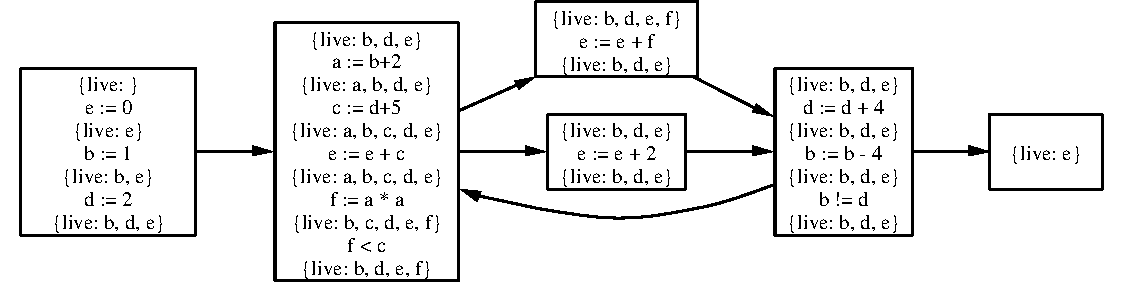
\includegraphics[scale=0.85]{livevars}
\end{center}

The register interference graph can then be determined based on which
pairs of variables are live simultaneously.
\begin{center}
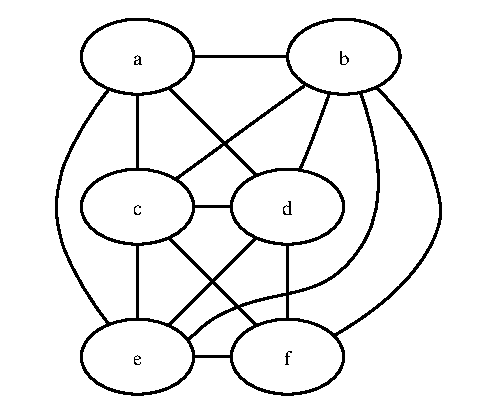
\includegraphics{regint}
\end{center}

\item
Suppose that the following Cool program is executed.
\begin{verbatim}
class C {
  x : C; y : C;
  setx(newx : C) : C { x <- newx };
  sety(newy : C) : C { y <- newy };
  setxy(newx : C, newy : C) : SELF_TYPE { { x <- newx; y <- newy; self; } }; };
class Main {
  x : C;
  main() : Object {
    let a : C <- new C, b : C <- new C, c : C <- new C, d : C <- new C,
        e : C <- new C, f : C <- new C, g : C <- new C, h : C <- new C in {
      f.sety(g); a.setxy(e, c); b.setx(f); g.setxy(f, d); c.sety(h); h.setxy(e, a);
      x <- c;
  } }; };
\end{verbatim}

\begin{enumerate}
\item
Draw the heap at the end of the execution of the program, identifying
objects by the names to which they are bound in the \texttt{let}
expression.  Assume that the root is the \texttt{Main} object created
at the start of the program, and that this object is not in the heap.
If the value of an attribute is \texttt{void}, don't show that
attribute as a pointer on the diagram.

The heap is shown below.  The only object pointed to by the roots is
\texttt{c}.
\begin{center}
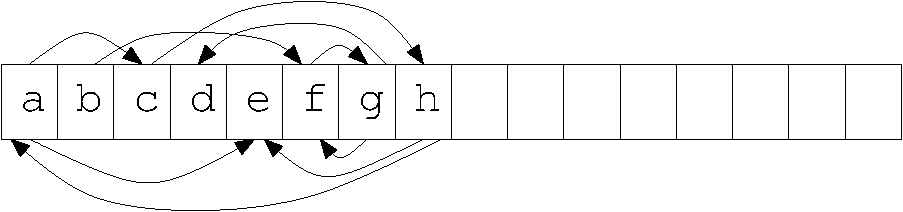
\includegraphics{heap}
\end{center}

\item
For each of the garbage collection algorithms discussed in class (Mark
and Sweep, Stop and Copy, and Reference Counting), show the heap after
garbage collection.  When the pointers of an object are processed,
assume that the processing order is the order of the attributes in the
source program.  Assume that the heap has space for at least $16$
objects.

In each of the following heap diagrams, the only object pointed to by
the roots is \texttt{c}.

\begin{itemize}
\item
Mark and Sweep
\begin{center}
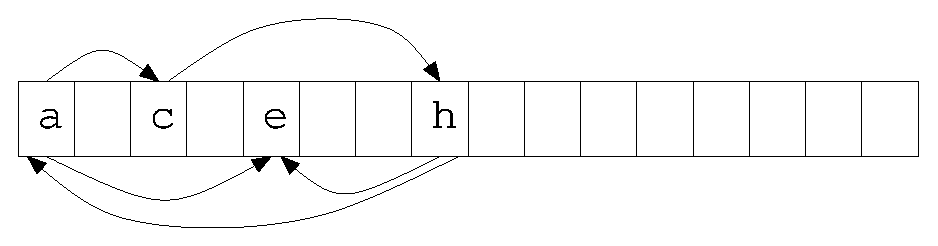
\includegraphics{marksweep}
\end{center}

All of the slots in the heap not occupied by objects are on the free
list.

\item
Stop and Copy
\begin{center}
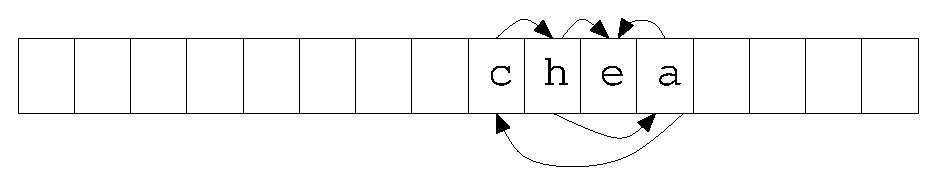
\includegraphics{stopcopy}
\end{center}

Note that object \texttt{e} appears before object \texttt{a} in the
new heap because the pointers of \texttt{h} are processed in the order
in which the attributes appear in the source text.

\item
Reference Counting
\begin{center}
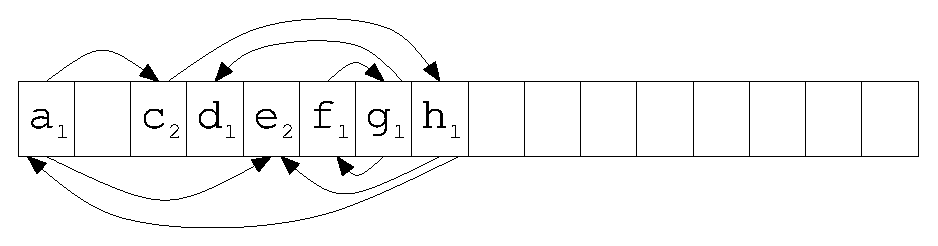
\includegraphics{refcount}
\end{center}

The diagram shows the reference count for each object.  The pointer
from the roots to the object \texttt{c} is counted as a reference for
\texttt{c}.
\end{itemize}
\end{enumerate}

\end{enumerate}

\end{document}
